\section{$\theta$の設定}

\begin{figure}[ht]
	\begin{center}
		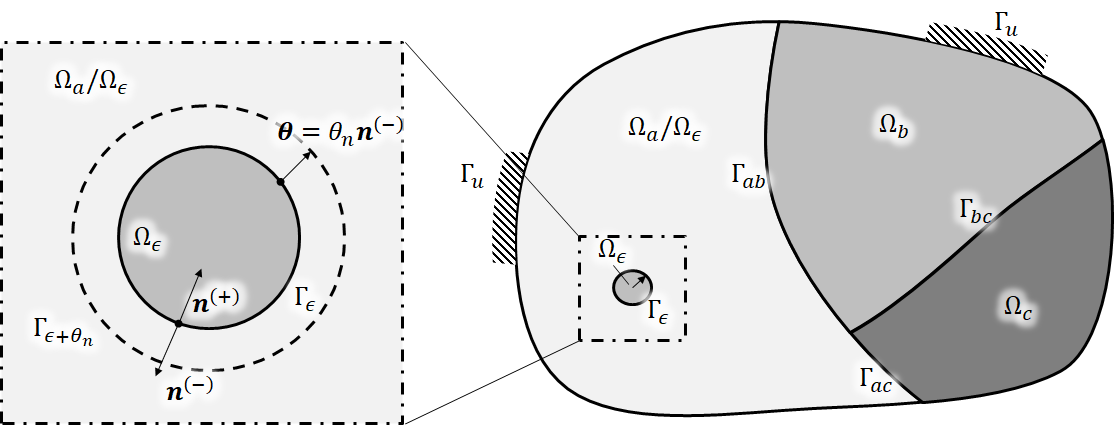
\includegraphics[width=13cm]{./figures/SDforTD.png}
		\caption{Topological derivative}
		\label{fig:TD}
	\end{center}
\end{figure}

$\bm{\theta}$を次式のように設定する
\begin{align}
	\bm{\theta}=\theta_{n}\bm{n}^{(-)}\hspace{1cm}\text{on}\hspace{0.3cm}\Gamma_{\epsilon}
\end{align}
この時,固有値$\lambda$の形状微分は,\eqref{eq:shape_lambda}に
$\bm{u}=\bm{u}^{\epsilon},\lambda=\lambda^{\epsilon}$を代入することで以下のようになる.
\begin{align}
	&\hspace{0.5cm}D\lambda(\Omega_{p\{1\leq p\leq n\}})\cdot\bm{\theta}
	\nonumber
	\\
	=&\int_{\Gamma_\epsilon}(\theta_{n}n_{m}^{(-)}n_{m}^{(-)})
	\Bigr(u_{i,j}^{\epsilon(-)}C_{ijkl}^{b}u_{k,l}^{\epsilon(-)}
	-\lambda^{\epsilon}\rho^{b}u_{i}^{\epsilon(-)}u_{i}^{\epsilon(-)}\Bigl) d\Omega
	\nonumber
	\\
	&+\int_{\Gamma_\epsilon}(\theta_{n}n_{m}^{(-)}n_{m}^{(+)})
	\Bigr(u_{i,j}^{\epsilon(+)}C_{ijkl}^{a}u_{k,l}^{\epsilon(+)}
	-\lambda^{\epsilon}\rho^{a}u_{i}^{\epsilon(+)}u_{i}^{\epsilon(+)}\Bigl) d\Omega
	\nonumber
	\\
	&-\int_{\Gamma_{\epsilon}}(\theta_{n}n_{m}^{(-)}n_{m}^{(-)})
	\Bigr(C_{ijkl}^{b}u_{k,l}^{\epsilon(-)}n_{j}^{(-)}
	-C_{ijkl}^{a}u_{k,l}^{\epsilon(+)}n_{j}^{(+)}\Bigl)
	(u_{i,\gamma}^{\epsilon(-)}n_\gamma^{(-)}-u_{i,\gamma}^{\epsilon(+)}n_\gamma^{(-)}) d\Gamma
	\nonumber
	\\
	=&\theta_{n}\int_{\Gamma_\epsilon}
	\Bigr(u_{i,j}^{\epsilon(-)}C_{ijkl}^{b}u_{k,l}^{\epsilon(-)}
	-\lambda^{\epsilon}\rho^{b}u_{i}^{\epsilon(-)}u_{i}^{\epsilon(-)}\Bigl) d\Omega
	\nonumber
	\\
	&-\theta_{n}\int_{\Gamma_\epsilon}
	\Bigr(u_{i,j}^{\epsilon(+)}C_{ijkl}^{a}u_{k,l}^{\epsilon(+)}
	-\lambda^{\epsilon}\rho^{a}u_{i}^{\epsilon(+)}u_{i}^{\epsilon(+)}\Bigl) d\Omega
	\nonumber
	\\
	&-\theta_{n}\int_{\Gamma_{\epsilon}}
	\Bigr(C_{ijkl}^{b}u_{k,l}^{\epsilon(-)}n_{j}^{(-)}
	+C_{ijkl}^{a}u_{k,l}^{\epsilon(+)}n_{j}^{(-)}\Bigl)
	(u_{i,\gamma}^{\epsilon(-)}n_\gamma^{(-)}-u_{i,\gamma}^{\epsilon(+)}n_\gamma^{(-)}) d\Gamma
	\label{eq:SDForTD}
\end{align}
ここで,
\begin{align}
	x_{1}-x_{1_{0}}=R\cos(\theta)
	\nonumber
	\\
	x_{2}-x_{2_{0}}=R\sin(\theta)
	\label{eq:xyToRTh}
\end{align}
と座標変換すると$R,\theta$方向の変位は以下のようになる.
\begin{align}
	u_{R}^{\epsilon(-)}(R,\theta)=&u_{x_{1}}(\bm{x}_{0})\cos(\theta)+u_{x_{2}}(\bm{x}_{0})\sin(\theta)
	+\epsilon\hat{w}_{r}^{(I\hspace{-.15em}I-)}(r,\theta)+O(\epsilon^2)
	\nonumber
	\\
	u_{\theta}^{\epsilon(-)}(R,\theta)=&-u_{x_{1}}(\bm{x}_{0})\sin(\theta)+u_{x_{2}}(\bm{x}_{0})\cos(\theta)
	+\epsilon\hat{w}_{\theta}^{(I\hspace{-.15em}I-)}(r,\theta)+O(\epsilon^2)
	\nonumber
	\\
	u_{R}^{\epsilon(+)}(R,\theta)=&u_{x_{1}}(\bm{x})\cos(\theta)+u_{x_{2}}(\bm{x})\sin(\theta)
	+\epsilon\hat{w}_{r}^{(I\hspace{-.15em}I+)}(r,\theta)+O(\epsilon^2)
	\nonumber
	\\
	u_{\theta}^{\epsilon(+)}(R,\theta)=&-u_{x_{1}}(\bm{x})\sin(\theta)+u_{x_{2}}(\bm{x})\cos(\theta)
	+\epsilon\hat{w}_{\theta}^{(I\hspace{-.15em}I+)}(r,\theta)+O(\epsilon^2)
	\label{eq:SDForTD}
\end{align}
歪みは以下のようになる.
\begin{align}
	e_{RR}^{\epsilon(-)}
		=&\frac{\partial u_{R}^{\epsilon(-)}}{\partial R}
		\nonumber
		\\
		=&\epsilon\frac{1}{\epsilon}\frac{\partial\hat{w}_{r}^{(I\hspace{-.15em}I-)}}{\partial r}(r,\theta)+O(\epsilon)
		\nonumber
		\\
		=&\frac{\partial\hat{w}_{r}^{(I\hspace{-.15em}I-)}}{\partial r}(r,\theta)+O(\epsilon)
		\label{eq:eRRInEps}
\end{align}
\begin{align}
	e_{R\theta}^{\epsilon(-)}
		=&\frac{1}{2}\Bigl( \frac{1}{R}\frac{\partial u_{R}^{\epsilon(-)}}{\partial \theta}
			+\frac{\partial u_{\theta}^{\epsilon(-)}}{\partial R}-\frac{u_{\theta}^{\epsilon(-)}}{R}\Bigr)
		\nonumber
		\\
		=&\frac{1}{2}\Bigl( \frac{1}{r}\frac{\partial \hat{w}_{r}^{(I\hspace{-.15em}I-)}}{\partial \theta}
			+\frac{\partial \hat{w}_{\theta}^{(I\hspace{-.15em}I-)}}{\partial r}
			-\frac{\hat{w}_{\theta}^{(I\hspace{-.15em}I-)}}{r}\Bigr)+O(\epsilon)
\end{align}
\begin{align}
	e_{\theta\theta}^{\epsilon(-)}
		=&\frac{1}{R}\frac{\partial u_{\theta}^{\epsilon(-)}}{\partial \theta}
			+\frac{u_{R}^{\epsilon(-)}}{R}
		\nonumber
		\\
		=&\frac{1}{r}\frac{\partial \hat{w}_{\theta}^{(I\hspace{-.15em}I-)}}{\partial \theta}
			+\frac{\hat{w}_{r}^{(I\hspace{-.15em}I-)}}{r}+O(\epsilon)
\end{align}
\begin{align}
	e_{RR}^{\epsilon(+)}
		=&\frac{\partial u_{R}^{\epsilon(+)}}{\partial R}
		\nonumber
		\\
		=&\Bigl\{ \frac{\partial u_{x_{1}}}{\partial x_{1}}(\bm{x})\cos(\theta)
			+\frac{\partial u_{x_{1}}}{\partial x_{2}}(\bm{x})\sin(\theta)\Bigr\}\cos(\theta)
		\nonumber
		\\
		&+\Bigl\{ \frac{\partial u_{x_{2}}}{\partial x_{1}}(\bm{x})\cos(\theta)
			+\frac{\partial u_{x_{2}}}{\partial x_{2}}(\bm{x})\sin(\theta)\Bigr\}\sin(\theta)
		+\epsilon\frac{1}{\epsilon}\frac{\partial\hat{w}_{r}^{(I\hspace{-.15em}I+)}}{\partial r}(r,\theta)+O(\epsilon)
		\nonumber
		\\
		=&\frac{1}{2}\Bigl\{ \frac{\partial u_{x_{1}}}{\partial x_{1}}(\bm{x})
			+\frac{\partial u_{x_{2}}}{\partial x_{2}}(\bm{x})\Bigr\}
		+\frac{1}{2}\Bigl\{ \frac{\partial u_{x_{1}}}{\partial x_{1}}(\bm{x})
			-\frac{\partial u_{x_{2}}}{\partial x_{2}}(\bm{x})\Bigr\}\cos(2\theta)
		\nonumber
		\\
		&+\frac{1}{2}\Bigl\{ \frac{\partial u_{x_{1}}}{\partial x_{2}}(\bm{x})
			+\frac{\partial u_{x_{2}}}{\partial x_{1}}(\bm{x})\Bigr\}\sin(2\theta)
		+\frac{\partial\hat{w}_{r}^{(I\hspace{-.15em}I+)}}{\partial r}(r,\theta)+O(\epsilon)
		\label{eq:eRROutEps}
\end{align}
\begin{align}
	e_{R\theta}^{\epsilon(+)}
		=&\frac{1}{2}\Bigl( \frac{1}{R}\frac{\partial u_{R}^{\epsilon(+)}}{\partial \theta}
			+\frac{\partial u_{\theta}^{\epsilon(+)}}{\partial R}-\frac{u_{\theta}^{\epsilon(+)}}{R}\Bigr)
		\nonumber
		\\
		=&\frac{1}{2}\Bigl[ \frac{1}{R}\bigl\{-u_{x1}(\bm{x})\sin(\theta)
				+u_{x2}(\bm{x})\cos(\theta)\bigr\}
			+\Bigl\{ -\frac{\partial u_{x_{1}}}{\partial x_{1}}(\bm{x})\sin(\theta)
				+\frac{\partial u_{x_{1}}}{\partial x_{2}}(\bm{x})\cos(\theta)\Bigr\}\cos(\theta)
			\nonumber
			\\
			&+\Bigl\{ -\frac{\partial u_{x_{2}}}{\partial x_{1}}(\bm{x})\sin(\theta)
				+\frac{\partial u_{x_{2}}}{\partial x_{2}}(\bm{x})\cos(\theta)\Bigr\}\sin(\theta)
			-\Bigl\{ \frac{\partial u_{x_{1}}}{\partial x_{1}}(\bm{x})\cos(\theta)
				+\frac{\partial u_{x_{1}}}{\partial x_{2}}(\bm{x})\sin(\theta)\Bigr\}\sin(\theta)
			\nonumber
			\\
			&+\Bigl\{ \frac{\partial u_{x_{2}}}{\partial x_{1}}(\bm{x})\cos(\theta)
				+\frac{\partial u_{x_{2}}}{\partial x_{2}}(\bm{x})\sin(\theta)\Bigr\}\cos(\theta)
			-\frac{1}{R}\bigl\{-u_{x1}(\bm{x})\sin(\theta)+u_{x2}(\bm{x})\cos(\theta)\bigr\}\Bigr]
			\nonumber
			\\
		&+\frac{1}{2}\Bigl( \frac{1}{r}\frac{\partial \hat{w}_{r}^{(I\hspace{-.15em}I-)}}{\partial \theta}
			+\frac{\partial \hat{w}_{\theta}^{(I\hspace{-.15em}I-)}}{\partial r}
			-\frac{\hat{w}_{\theta}^{(I\hspace{-.15em}I-)}}{r}\Bigr)+O(\epsilon)
		\nonumber
		\\
		=&-\frac{1}{2}\Bigl\{ \frac{\partial u_{x_{1}}}{\partial x_{1}}(\bm{x})
			-\frac{\partial u_{x_{2}}}{\partial x_{2}}(\bm{x})\Bigr\}\sin(2\theta)
		+\frac{1}{2}\Bigl\{ \frac{\partial u_{x_{1}}}{\partial x_{2}}(\bm{x})
			+\frac{\partial u_{x_{2}}}{\partial x_{1}}(\bm{x})\Bigr\}\cos(2\theta)
			\nonumber
			\\
		&+\frac{1}{2}\Bigl( \frac{1}{r}\frac{\partial \hat{w}_{r}^{(I\hspace{-.15em}I+)}}{\partial \theta}
			+\frac{\partial \hat{w}_{\theta}^{(I\hspace{-.15em}I+)}}{\partial r}
			-\frac{\hat{w}_{\theta}^{(I\hspace{-.15em}I+)}}{r}\Bigr)+O(\epsilon)
\end{align}
\begin{align}
	e_{\theta\theta}^{\epsilon(+)}
		=&\frac{1}{R}\frac{\partial u_{\theta}^{\epsilon(+)}}{\partial \theta}
			+\frac{u_{R}^{\epsilon(+)}}{R}
		\nonumber
		\\
		=&\frac{1}{R}\bigl\{-u_{x_{1}}(\bm{x})\cos(\theta)-u_{x_{2}}(\bm{x})\sin(\theta)\bigr\}
		-\Bigl\{ -\frac{\partial u_{x_{1}}}{\partial x_{1}}(\bm{x})\sin(\theta)
			+\frac{\partial u_{x_{1}}}{\partial x_{2}}(\bm{x})\cos(\theta)\Bigr\}\sin(\theta)
		\nonumber
		\\
		&+\Bigl\{ -\frac{\partial u_{x_{2}}}{\partial x_{1}}(\bm{x})\sin(\theta)
			+\frac{\partial u_{x_{2}}}{\partial x_{2}}(\bm{x})\cos(\theta)\Bigr\}\cos(\theta)
		+\frac{1}{R}\bigl\{u_{x_{1}}(\bm{x})\cos(\theta)u_{x_{2}}(\bm{x})\sin(\theta)\bigr\}
		\nonumber
		\\
		=&\frac{1}{2}\Bigl\{ \frac{\partial u_{x_{1}}}{\partial x_{1}}(\bm{x})
			+\frac{\partial u_{x_{2}}}{\partial x_{2}}(\bm{x})\Bigr\}
		-\frac{1}{2}\Bigl\{ \frac{\partial u_{x_{1}}}{\partial x_{1}}(\bm{x})
			-\frac{\partial u_{x_{2}}}{\partial x_{2}}(\bm{x})\Bigr\}\cos(2\theta)
		\nonumber
		\\
		&-\frac{1}{2}\Bigl\{ \frac{\partial u_{x_{1}}}{\partial x_{2}}(\bm{x})
			+\frac{\partial u_{x_{2}}}{\partial x_{1}}(\bm{x})\Bigr\}\sin(2\theta)
		+\frac{1}{r}\frac{\partial \hat{w}_{\theta}^{(I\hspace{-.15em}I+)}}{\partial \theta}
			+\frac{\hat{w}_{r}^{(I\hspace{-.15em}I+)}}{r}+O(\epsilon)
	\label{eq:eThThOutEps}
\end{align}

$\Gamma_\epsilon$上での歪みは以下のようになる.
\begin{align}
	e_{RR}^{\epsilon(-)}
	=&\frac{\mu^{a}\kappa^{a}}{2\bigl(\mu^{a}(\kappa^{b}-1)+2\mu^{b}\bigr)}
	\bigl\{u_{x_{1},x_{1}}(\bm{x_{0}})+u_{x_{2},x_{2}}(\bm{x_{0}})\bigr\}
	\nonumber
	\\
	&+\frac{\mu^{a}\bigl(\kappa^{a}+1\bigr)}{2\bigl(\mu^{a}+\kappa^{a}\mu^{b}\bigr)}
	\bigl\{u_{x_{1},x_{1}}(\bm{x_{0}})-u_{x_{2},x_{2}}(\bm{x_{0}})\bigr\}\cos(2\theta)
	\nonumber
	\\
	&+\frac{\mu^{a}\bigl(\kappa^{a}+1\bigr)}{2\bigl(\mu^{a}+\kappa^{a}\mu^{b}\bigr)}
	\bigl\{u_{x_{1},x_{2}}(\bm{x_{0}})+u_{x_{2},x_{1}}(\bm{x_{0}})\bigr\}\sin(2\theta)
	\label{eq:eRRInEpsSol}
\end{align}
\begin{align}
	e_{R\theta}^{\epsilon(-)}
	=&-\frac{\mu^{a}\bigl(\kappa^{a}+1\bigr)}{2\bigl(\mu^{a}+\kappa^{a}\mu^{b}\bigr)}
	\bigl\{u_{x_{1},x_{1}}(\bm{x_{0}})-u_{x_{2},x_{2}}(\bm{x_{0}})\bigr\}\sin(2\theta)
	\nonumber
	\\
	&+\frac{\mu^{a}\bigl(\kappa^{a}+1\bigr)}{2\bigl(\mu^{a}+\kappa^{a}\mu^{b}\bigr)}
	\bigl\{u_{x_{1},x_{2}}(\bm{x_{0}})+u_{x_{2},x_{1}}(\bm{x_{0}})\bigr\}\cos(2\theta)
	\label{eq:eRThInEpsSol}
\end{align}
\begin{align}
	e_{\theta\theta}^{\epsilon(-)}
	=&\frac{\mu^{a}\kappa^{a}}{2\bigl(\mu^{a}(\kappa^{b}-1)+2\mu^{b}\bigr)}
	\bigl\{u_{x_{1},x_{1}}(\bm{x_{0}})+u_{x_{2},x_{2}}(\bm{x_{0}})\bigr\}
	\nonumber
	\\
	&-\frac{\mu^{a}\bigl(\kappa^{a}+1\bigr)}{2\bigl(\mu^{a}+\kappa^{a}\mu^{b}\bigr)}
	\bigl\{u_{x_{1},x_{1}}(\bm{x_{0}})-u_{x_{2},x_{2}}(\bm{x_{0}})\bigr\}\cos(2\theta)
	\nonumber
	\\
	&-\frac{\mu^{a}\bigl(\kappa^{a}+1\bigr)}{2\bigl(\mu^{a}+\kappa^{a}\mu^{b}\bigr)}
	\bigl\{u_{x_{1},x_{2}}(\bm{x_{0}})+u_{x_{2},x_{1}}(\bm{x_{0}})\bigr\}\sin(2\theta)
	\label{eq:eThThInEpsSol}
\end{align}

%外側の歪み
\begin{align}
	e_{RR}^{\epsilon(+)}
	=&\frac{ \mu^{a}\bigl(\kappa^{b}-1\bigr)\bigl(\kappa^{a}-2\bigr)+4\mu^{b}\bigl(\kappa^{a}-1\bigr) }
		{2\bigl(\mu^{a}(\kappa^{b}-1)+2\mu^{b}\bigr)(\kappa^{a}-1)}
	\bigl\{u_{x_{1},x_{1}}(\bm{x_{0}})+u_{x_{2},x_{2}}(\bm{x_{0}})\bigr\}
	\nonumber
	\\
	&+\frac{\mu^{a}\bigl(3-\kappa^{a}\bigr)+2\mu^{b}\bigl(\kappa^{a}-1\bigr)}{2\bigl(\mu^{a}+\kappa^{a}\mu^{b}\bigr)}
	\bigl\{u_{x_{1},x_{1}}(\bm{x_{0}})-u_{x_{2},x_{2}}(\bm{x_{0}})\bigr\}\cos(2\theta)
	\nonumber
	\\
	&+\frac{\mu^{a}\bigl(3-\kappa^{a}\bigr)+2\mu^{b}\bigl(\kappa^{a}-1\bigr)}{2\bigl(\mu^{a}+\kappa^{a}\mu^{b}\bigr)}
	\bigl\{u_{x_{1},x_{2}}(\bm{x_{0}})+u_{x_{2},x_{1}}(\bm{x_{0}})\bigr\}\sin(2\theta)
	\label{eq:eRROutEpsSol}
\end{align}
\begin{align}
	e_{R\theta}^{\epsilon(+)}
	=&\frac{\mu^{a}-\mu^{b}\bigl(\kappa^{a}+2\bigr)}{\mu^{a}+\kappa^{a}\mu^{b}}
	\bigl\{u_{x_{1},x_{1}}(\bm{x_{0}})-u_{x_{2},x_{2}}(\bm{x_{0}})\bigr\}\sin(2\theta)
	\nonumber
	\\
	&-\frac{\mu^{a}-\mu^{b}\bigl(\kappa^{a}+2\bigr)}{\mu^{a}+\kappa^{a}\mu^{b}}
	\bigl\{u_{x_{1},x_{2}}(\bm{x_{0}})+u_{x_{2},x_{1}}(\bm{x_{0}})\bigr\}\cos(2\theta)
	\label{eq:eRThOutEpsSol}
\end{align}
\begin{align}
	e_{\theta\theta}^{\epsilon(+)}
	=&\frac{\mu^{a}\kappa^{a}(\kappa^{b}-1)}
	{2\bigl(\mu^{a}(\kappa^{b}-1)+2\mu^{b}\bigr)(\kappa^{a}-1)}
	\bigl\{u_{x_{1},x_{1}}(\bm{x_{0}})+u_{x_{2},x_{2}}(\bm{x_{0}})\bigr\}
	\nonumber
	\\
	&-\frac{\mu^{a}\bigl(\kappa^{a}+1\bigr)-2\kappa^{a}\mu^{b}}{2\bigl(\mu^{a}+\kappa^{a}\mu^{b}\bigr)}
	\bigl\{u_{x_{1},x_{1}}(\bm{x_{0}})-u_{x_{2},x_{2}}(\bm{x_{0}})\bigr\}\cos(2\theta)
	\nonumber
	\\
	&-\frac{\mu^{a}\bigl(\kappa^{a}+1\bigr)-2\kappa^{a}\mu^{b}}{2\bigl(\mu^{a}+\kappa^{a}\mu^{b}\bigr)}
	\bigl\{u_{x_{1},x_{2}}(\bm{x_{0}})+u_{x_{2},x_{1}}(\bm{x_{0}})\bigr\}\sin(2\theta)
	\label{eq:eThThOutEpsSol}
\end{align}
歪みと応力の関係\eqref{eq:Constitute2}より,応力は以下のようになる.
\begin{align}
	\sigma_{RR}
	=&\frac{\kappa+1}{\kappa-1}\mu e_{RR}^{}+\frac{3-\kappa}{\kappa-1}\mu e_{\theta\theta}^{}
	\nonumber
	\\
	\sigma_{\theta\theta}
	=&\frac{\kappa+1}{\kappa-1}\mu e_{\theta\theta}^{}+\frac{3-\kappa}{\kappa-1}\mu e_{RR}^{}
	\nonumber
	\\
	\sigma_{R\theta}=&2\mu e_{R\theta}^{}
	\label{eq:Constitute2}
\end{align}

\begin{align}
	\sigma_{RR}^{\epsilon(-)} =
	&\frac{2\mu^{a}\mu^{b}\kappa^{a}}{\bigl(\mu^{a}(\kappa^{b}-1)+2\mu^{b}\bigr)(\kappa^{a}-1)}
	\bigl\{u_{x_{1},x_{1}}(\bm{x_{0}})+u_{x_{2},x_{2}}(\bm{x_{0}})\bigr\}
	\nonumber
	\\
	&+\frac{\mu^{a}\mu^{b}\bigl(\kappa^{a}+1\bigr)}{\mu^{a}+\kappa^{a}\mu^{b}}
	\bigl\{u_{x_{1},x_{1}}(\bm{x_{0}})-u_{x_{2},x_{2}}(\bm{x_{0}})\bigr\}\cos(2\theta)
	\nonumber
	\\
	&+\frac{\mu^{a}\mu^{b}\bigl(\kappa^{a}+1\bigr)}{\mu^{a}+\kappa^{a}\mu^{b}}
	\bigl\{u_{x_{1},x_{2}}(\bm{x_{0}})+u_{x_{2},x_{1}}(\bm{x_{0}})\bigr\}\sin(2\theta)
	\label{eq:SigmaRRInEpsSol}
\end{align}
\begin{align}
	\sigma_{R\theta}^{\epsilon(-)} =
	&-\frac{\mu^{a}\mu^{b}\bigl(\kappa^{a}+1\bigr)}{\mu^{a}+\kappa^{a}\mu^{b}}
	\bigl\{u_{x_{1},x_{1}}(\bm{x_{0}})-u_{x_{2},x_{2}}(\bm{x_{0}})\bigr\}\sin(2\theta)
	\nonumber
	\\
	&+\frac{\mu^{a}\mu^{b}\bigl(\kappa^{a}+1\bigr)}{\mu^{a}+\kappa^{a}\mu^{b}}
	\bigl\{u_{x_{1},x_{2}}(\bm{x_{0}})+u_{x_{2},x_{1}}(\bm{x_{0}})\bigr\}\cos(2\theta)
	\label{eq:SigmaRThInEpsSol}
\end{align}
\begin{align}
	\sigma_{\theta\theta}^{\epsilon(-)} =
	&\frac{2\mu^{a}\mu^{b}\kappa^{a}}{\bigl(\mu^{a}(\kappa^{b}-1)+2\mu^{b}\bigr)(\kappa^{a}-1)}
	\bigl\{u_{x_{1},x_{1}}(\bm{x_{0}})+u_{x_{2},x_{2}}(\bm{x_{0}})\bigr\}
	\nonumber
	\\
	&-\frac{\mu^{a}\mu^{b}\bigl(\kappa^{a}+1\bigr)}{\mu^{a}+\kappa^{a}\mu^{b}}
	\bigl\{u_{x_{1},x_{1}}(\bm{x_{0}})-u_{x_{2},x_{2}}(\bm{x_{0}})\bigr\}\cos(2\theta)
	\nonumber
	\\
	&-\frac{\mu^{a}\mu^{b}\bigl(\kappa^{a}+1\bigr)}{\mu^{a}+\kappa^{a}\mu^{b}}
	\bigl\{u_{x_{1},x_{2}}(\bm{x_{0}})+u_{x_{2},x_{1}}(\bm{x_{0}})\bigr\}\sin(2\theta)
	\label{eq:SigmaThThInEpsSol}
\end{align}

\begin{align}
	\sigma_{RR}^{\epsilon(+)}
	=&\frac{ \mu^{a}\{\mu^{a}\bigl(\kappa^{b}-1\bigr)+2\mu^{b}\bigl(\kappa^{a}+1\bigr)\} }
		{\bigl(\mu^{a}(\kappa^{b}-1)+2\mu^{b}\bigr)(\kappa^{a}-1)}
	\bigl\{u_{x_{1},x_{1}}(\bm{x_{0}})+u_{x_{2},x_{2}}(\bm{x_{0}})\bigr\}
	\nonumber
	\\
	&+\frac{\mu^{a}\bigl(3-\kappa^{a}\bigr)+2\mu^{b}\bigl(\kappa^{a}-1\bigr)}{2\bigl(\mu^{a}+\kappa^{a}\mu^{b}\bigr)}
	\bigl\{u_{x_{1},x_{1}}(\bm{x_{0}})-u_{x_{2},x_{2}}(\bm{x_{0}})\bigr\}\cos(2\theta)
	\nonumber
	\\
	&+\frac{\mu^{a}\bigl(3-\kappa^{a}\bigr)+2\mu^{b}\bigl(\kappa^{a}-1\bigr)}{2\bigl(\mu^{a}+\kappa^{a}\mu^{b}\bigr)}
	\bigl\{u_{x_{1},x_{2}}(\bm{x_{0}})+u_{x_{2},x_{1}}(\bm{x_{0}})\bigr\}\sin(2\theta)
	\label{eq:eRROutEpsSol}
\end{align}
\begin{align}
	\sigma_{R\theta}^{\epsilon(+)}
	=&\frac{\mu^{a}-\mu^{b}\bigl(\kappa^{a}+2\bigr)}{\mu^{a}+\kappa^{a}\mu^{b}}
	\bigl\{u_{x_{1},x_{1}}(\bm{x_{0}})-u_{x_{2},x_{2}}(\bm{x_{0}})\bigr\}\sin(2\theta)
	\nonumber
	\\
	&-\frac{\mu^{a}-\mu^{b}\bigl(\kappa^{a}+2\bigr)}{\mu^{a}+\kappa^{a}\mu^{b}}
	\bigl\{u_{x_{1},x_{2}}(\bm{x_{0}})+u_{x_{2},x_{1}}(\bm{x_{0}})\bigr\}\cos(2\theta)
	\label{eq:eRThOutEpsSol}
\end{align}
\begin{align}
	\sigma_{\theta\theta}^{\epsilon(+)}
	=&\frac{\mu^{a}\kappa^{a}(\kappa^{b}-1)}
	{2\bigl(\mu^{a}(\kappa^{b}-1)+2\mu^{b}\bigr)(\kappa^{a}-1)}
	\bigl\{u_{x_{1},x_{1}}(\bm{x_{0}})+u_{x_{2},x_{2}}(\bm{x_{0}})\bigr\}
	\nonumber
	\\
	&-\frac{\mu^{a}\bigl(\kappa^{a}+1\bigr)-2\kappa^{a}\mu^{b}}{2\bigl(\mu^{a}+\kappa^{a}\mu^{b}\bigr)}
	\bigl\{u_{x_{1},x_{1}}(\bm{x_{0}})-u_{x_{2},x_{2}}(\bm{x_{0}})\bigr\}\cos(2\theta)
	\nonumber
	\\
	&-\frac{\mu^{a}\bigl(\kappa^{a}+1\bigr)-2\kappa^{a}\mu^{b}}{2\bigl(\mu^{a}+\kappa^{a}\mu^{b}\bigr)}
	\bigl\{u_{x_{1},x_{2}}(\bm{x_{0}})+u_{x_{2},x_{1}}(\bm{x_{0}})\bigr\}\sin(2\theta)
	\label{eq:eThThOutEpsSol}
\end{align}
